\chapter{Introduction} \label{Introduction}

\section{Motivations}
% \todo{Expand upon this section}
Reliable access to electricity is a critical component of a prosperous society. Increasing access to energy in areas that lack that access \cite{international2022world}. Furthermore, given that electricity is foundational to economic growth and the maintenance of social services like education and healthcare \cite{owid-sdgs-affordable-clean-energy}, people remain interested in maintaining and increasing energy production and distribution. 

\section{Microgrids} \label{Introduction:Microgrid}
Microgrids, which consist of power sources servicing loads, exchange around 10 MVA of power \cite{Uddin_Microgrid_Scale, Trends_in_Microgrid} Microgrids operate using either DC, single-phase AC, or three-phase AC electricity \cite{Uddin_Microgrid_Scale}. By contrast, nanogrids, or systems that provide electrical power to a single building or small cluster of buildings, can have individual power ratings of approximately 10 kVA \cite{Pindoriya_Nanogrid_Rating}. Nanogrids typically operate using DC or single-phase AC electricity \cite{Jie_Nanogrid_Rating, Pindoriya_Nanogrid_Rating}. 

\subsection{Three-Phase AC Microgrids}

Three-phase AC microgrids typically service small industrial loads.

\textcolor{blue}{
\begin{itemize}
    \item Typical load size
    \item Locations
    \item Configuration (diagram)
\end{itemize}
}

\section{Connections between two Microgrids}

The interface of a microgrid into a power system typically consists of power electronic-based systems \cite{Barnes}. Bidirectional power transfer across these systems is typically a feature \cite{Deng}. Research is being undertaken to improve stability of microgrids, which are often conceptualized as relatively “weak” systems \cite{Rezaee}.

\subsection{Issues in Microgrid Interconnections}
Issues in microgrid interconnections include the following:
\begin{itemize}
    \item Interconnection transients
    \item Power allocation (energy management)
    \item Rapid Dynamics (to a greater extent than a microgrid-grid interconnection)
    \item Response to faults and other voltage imbalances 
\end{itemize}

\section{Problem Statement}

Considering two islanded microgrids supplying residential or light industrial loads, the broad research question is to explore how interconnecting these microgrids can improve their operation.

To explore this question, a minial microgrid power system is defined as a generator of fixed rating powering a load that can vary in demand. The central problem is: if an interconnection is placed between two such power systems and the load demand on one of the generators exceeds the capacity of the generator powering it, how can excess capacity from the other power system be used to relieve the first one?

\section{Research Objectives}

\subsection{Project Scope}

For validation of prototypes like the one being proposed in this work, it is typical that a much smaller scale system is used. Typical power ratings of prototype back-to-back converters have ranged from 1.5 kVA to 5 kVA \cite{Wu_Model_Size, Jung_Model_Size} and have worked with source voltages around 208 V at frequencies of 50-60 Hz \cite{Blaabjerg_Grid_Synchronization, Wu_Model_Size, Jung_Model_Size}, indicating that prototypes of that size have generally been effective at demonstrating that proposed concepts are valid. Thus, the chosen power rating of this project’s bidirectional converter is 5 kVA, and source voltages will be of 208 V at 60 Hz, as shown in \autoref{fig:Quick_Abstraction}. 

\begin{figure}
    \centering
    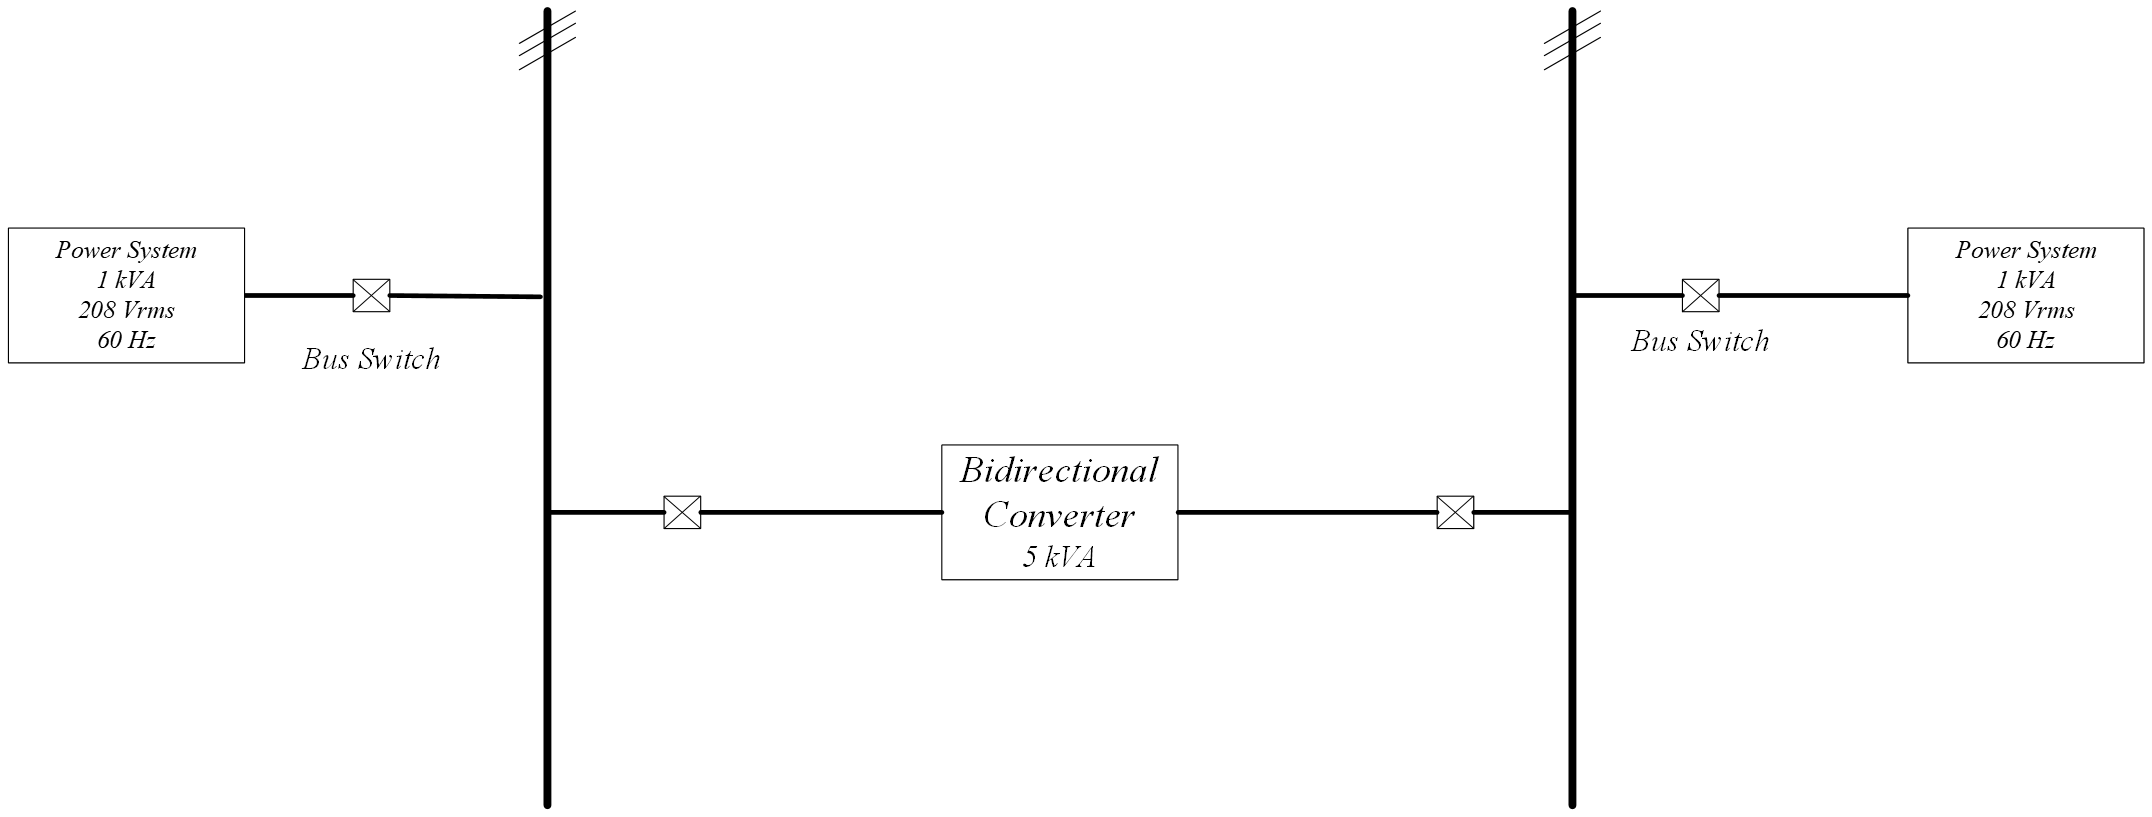
\includegraphics[width=0.95\linewidth]{Images/Quick_Abstraction_2024.11.11.png}
    \caption{High-level Model with System Power Ratings}
    \label{fig:Quick_Abstraction}
\end{figure}

\section{Contributions}

\textcolor{blue}{
\begin{itemize}
    \item Interconnection design for weak microgrids of particular size
    \item Validation using real-life objects
    \item Validation using particular switching scheme
\end{itemize}
}

\section{Thesis Organization}

The rest of this thesis is organized as follows. Chapter 2 deals with the theory of synchronization between two power systems with individual frequency, phase, and voltage characteristics. Chapter 3 discusses theoretical bases for the interconnection of two three-phase power systems. Chapter 4 simulates a potential experimental set-up to evaluate a potential interconnection. Chapter 5 discusses the experimental set-up to evaluate a potential interconnection. Chapter 6 evaluates the results of that experimental setup and discusses the implications. Chapter 7 concludes the thesis and explores bases for future work.